\section*{Introduction}

PixelToPosEstimator is a C library providing structures and functions to estimate 3D position from a 2D image.\\ 

The problem is as follow: given the 2D image of a set of points laying on a plane seen from a point of view, if we know the 3D position of the point of view and the 3D position and 2D position in the image of at least 3 points on the plane, how to estimate the 3D position of other points from their 2D position in the image.\\

PixelToPosEstimator provides a solution by using the known points to search the parameters optimizing a model of the projection from the 3D coordinates to the 2D coordinates, and then uses this optimized model to calculate other points. The optimization is performed using the \begin{ttfamily}GenAlg\end{ttfamily} library.\\

It uses the \begin{ttfamily}PBErr\end{ttfamily}, \begin{ttfamily}PBMath\end{ttfamily}, \begin{ttfamily}GSet\end{ttfamily}, \begin{ttfamily}GenAlg\end{ttfamily} libraries.\\

\section{Definitions}

The problem consists of finding the function $F()$ such as $\overrightarrow{R_p}=F(\overrightarrow{S_p})$, where $\overrightarrow{R_p}$ is the 3D coordinates of the point $p$ and $\overrightarrow{S_p}$ is the screen coordinates of the point $p$, shorten below as, respectively, $\overrightarrow{R}$, $\overrightarrow{S}$.\\

Screen coordinates system ($\overrightarrow{0},\overrightarrow{u},\overrightarrow{v}$) is as follow: $\overrightarrow{0}$ is at the top-left corner, $\overrightarrow{u}$ is toward the right and $\overrightarrow{v}$ is toward the bottom. Screen dimensions are noted $W$ for width and $H$ for height.\\

Lets define $\overrightarrow{P_p}$, the "polar" coordinates of the point $p$, shorten below as $\overrightarrow{P}$, as follow:\\
\begin{equation}
\overrightarrow{P}=\
\left\lbrace\begin{array}{l}
\frac{S_u-0.5W}{0.5W}\\
\frac{S_v-0.5H}{0.5H}\\
\end{array}\right.
\end{equation}
The polar coordinates represents the deviation of the point from the center of the screen relatively to the screen dimensions.\\

Lets now consider the projection of the screen on $\mathcal{S}$ the unit sphere centered on the camera position $\overrightarrow{C}$. The camera's orthonormal coordinates system is $(\overrightarrow{C},\overrightarrow{right},\overrightarrow{up},\overrightarrow{depth})$ such as $\overrightarrow{depth}$ is colinear to $\overrightarrow{CV}$, where $\overrightarrow{V}$ is the point of view of the camera.\\

if we note $\alpha$ and $\beta$ the angle of view of the camera along respectively $\overrightarrow{x}$ and $\overrightarrow{y}$, $\overrightarrow{P_{\mathcal{S}}}$ the projection of 
$\overrightarrow{S}$ on $\mathcal{S}$ is calculated as follow:\\
\begin{equation}
\overrightarrow{P'_{\mathcal{S}}}=Rot_{\overrightarrow{up}}(\overrightarrow{depth},\alpha P_x)+Rot_{\overrightarrow{right}}(\overrightarrow{depth},\beta P_y)-\overrightarrow{depth}
\end{equation}
\begin{equation}
\overrightarrow{P_{\mathcal{S}}}=\frac{\overrightarrow{P'_{\mathcal{S}}}}{||\overrightarrow{P'_{\mathcal{S}}}||}\\
\end{equation}
where $Rot_{\overrightarrow{w}}(\overrightarrow{A}, \theta)$ is the right-handed rotation of $\overrightarrow{A}$ around $\overrightarrow{w}$ by $\theta$ (in radians). We remind that the rotation matrix $M$ is equal to (to shorten notation $\theta$ is not written in the matrix below):\\
\begin{equation}
M=\left[
\begin{array}{ccc}
cos+w_x^2(1-cos)&w_xw_y(1-cos)-w_zsin&w_xw_z(1-cos)+w_ysin\\
w_xw_y(1-cos)+w_zsin&cos+w_y^2(1-cos)&w_yw_z(1-cos)-w_xsin\\
w_xw_z(1-cos)-w_ysin&w_yw_z(1-cos)+w_xsin&cos+w_z^2(1-cos)\\
\end{array}
\right]
\end{equation}

From $\overrightarrow{P_{\mathcal{S}}}$ it is then possible to calculate $\overrightarrow{R}$ as follow: it is the intersection of the line $(CP_{\mathcal{S}})$ and the plane $(\overrightarrow{x},\overrightarrow{z})$:\\
\begin{equation}
\overrightarrow{R}=\left.(\overrightarrow{C}+\gamma\overrightarrow{CP_{\mathcal{S}}})\right|_{C_y+\gamma ({P_{\mathcal{S}}}_y-C_y)=0}
\end{equation}
which gives us the expression of the searched function $F()$.\\

However, this function relies on several unknown values:\\
\begin{itemize}
\item $\overrightarrow{V}$ the point of view of the camera
\item $\alpha$ and $\beta$ the angle of view of the camera
\item $\overrightarrow{up}$ the up direction in the camera coordinates system. ($\overrightarrow{right}$ is not an unknown as we can calculate it as follow: $\overrightarrow{right}=\overrightarrow{depth}*\overrightarrow{up}$)
\end{itemize}

Then, given $\mathcal{I}$ the set of points for which we know both the 3D coordinates and 2D coordinates, we approximate these unknown values by solving the minimization problem:\\
\begin{equation}
\left\lbrace
\begin{array}{l}
{V_x,V_y,V_z,\alpha,\beta,up_x,up_y,up_z}\in\mathbb{R}^8\\
Min_{(\mathcal{I},\overrightarrow{V},\alpha,\beta,\overrightarrow{up})}(\frac{1}{\mathcal{I}^*}\sum_{i\in\mathcal{I}}||\overrightarrow{R_i}-F_{(\overrightarrow{V},\alpha,\beta,\overrightarrow{up})}(\overrightarrow{S_i})||)\\
\end{array}
\right.
\end{equation}

\section{Interface}

\begin{scriptsize}
\begin{ttfamily}
\verbatiminput{/home/bayashi/GitHub/PixelToPosEstimator/pixeltoposestimator.h}
\end{ttfamily}
\end{scriptsize}

\section{Code}

\subsection{pixeltoposestimator.c}

\begin{scriptsize}
\begin{ttfamily}
\verbatiminput{/home/bayashi/GitHub/PixelToPosEstimator/pixeltoposestimator.c}
\end{ttfamily}
\end{scriptsize}

\section{Makefile}

\begin{scriptsize}
\begin{ttfamily}
\verbatiminput{/home/bayashi/GitHub/PixelToPosEstimator/Makefile}
\end{ttfamily}
\end{scriptsize}

\section{Example}

\subsection{Test case}

\begin{scriptsize}
\begin{ttfamily}
\verbatiminput{/home/bayashi/GitHub/PixelToPosEstimator/ground.pov}
\end{ttfamily}
\end{scriptsize}

In the image below, the four input positions are in black, and the 2 test positions are in red. The red circles show the error range of the estimation.:\\
\begin{center}
\begin{figure}[H]
\centering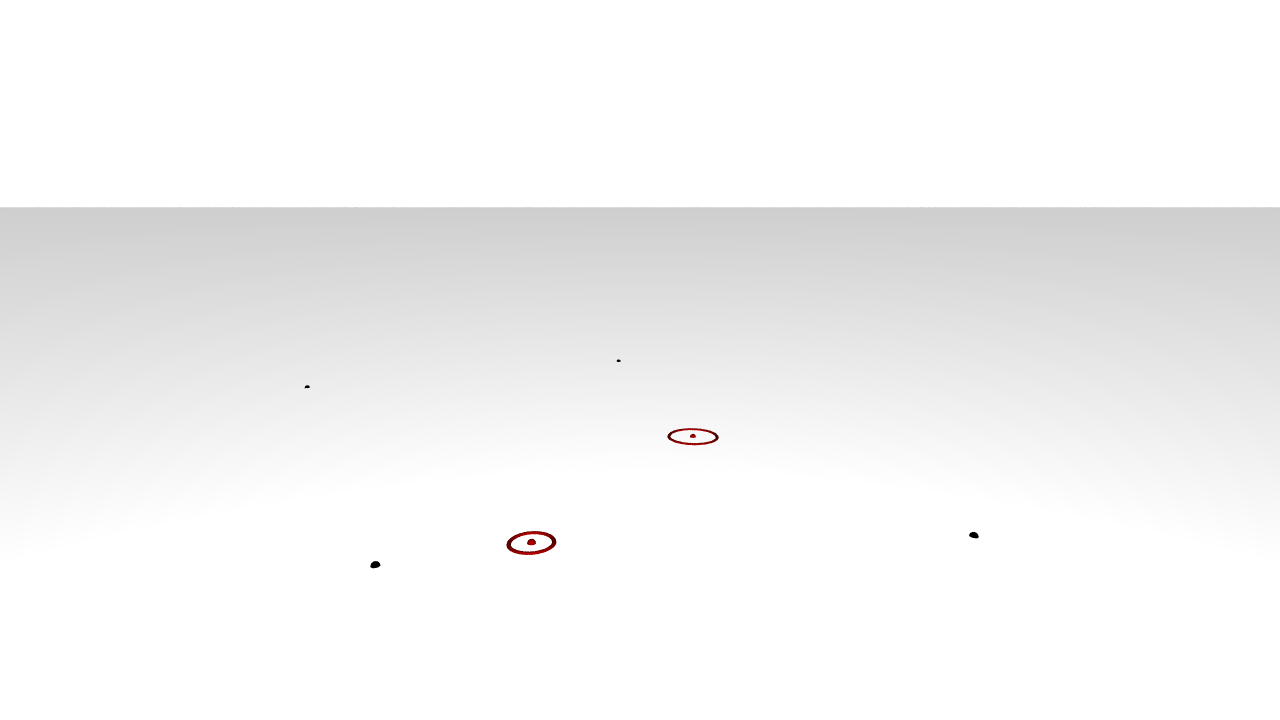
\includegraphics[width=6cm]{/home/bayashi/GitHub/PixelToPosEstimator/ground.png}\\
\end{figure}
\end{center}

\subsection{main.c}

\begin{scriptsize}
\begin{ttfamily}
\verbatiminput{/home/bayashi/GitHub/PixelToPosEstimator/main.c}
\end{ttfamily}
\end{scriptsize}

inputTest.txt:\\
\begin{scriptsize}
\begin{ttfamily}
\verbatiminput{/home/bayashi/GitHub/PixelToPosEstimator/inputTest.txt}
\end{ttfamily}
\end{scriptsize}

\section{Output}

\begin{scriptsize}
\begin{ttfamily}
\verbatiminput{/home/bayashi/GitHub/PixelToPosEstimator/res.txt}
\end{ttfamily}
\end{scriptsize}

\begin{center}
\begin{figure}[H]
\centering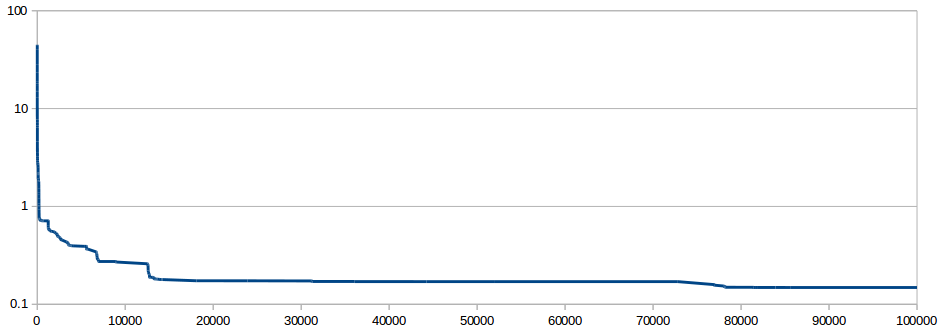
\includegraphics[width=6cm]{/home/bayashi/GitHub/PixelToPosEstimator/param.png}\\
\end{figure}
\end{center}

param.txt:\\
\begin{scriptsize}
\begin{ttfamily}
\verbatiminput{/home/bayashi/GitHub/PixelToPosEstimator/param.txt}
\end{ttfamily}
\end{scriptsize}


